% Chapter 4: Results

\chapter{Resultados} % Main chapter title

\label{Chapter4} % For referencing this chapter elsewhere, use \ref{Chapter4}

%-------------------------------------------------------------------------------

\section{Especificaciones del sistema}

En esta sección se detallan las especificaciones del sistema resultante tras desarrollo del proyecto. Se detallan las prestaciones de este, así como los modelos de datos finales, y las entradas y salidas.

\subsection{Definición y funcionalidades}

\textbf{Grimoirebots} es el resultado del desarrollo expuesto en el Capítulo~{\ref{Chapter3}}. Se trata de un complejo sistema de análisis de repositorios git que, de forma automática, obtiene y genera datos sobre el desarrollo de \emph{software}, permitiendo su uso mediante la creación de métricas y gráficas.

%-------------------------------------------------------------------------------

\section{Despliegue}

\subsection{Requisitos}

En esta sección se describen todas las herramientas y \emph{software}\index{Software} que es necesario instalar en el sistema antes de la ejecución de Grimoirebots.

\begin{itemize}
    \item \textbf{Docker}\index{Docker} -- La ejecución de Grimoirebots se realiza usando contenedores Docker, por lo que su instalación es obligatoria. La instalación de Docker es diferente en función del Sistema Operativo utilizado, encontrándose una guía para los más utilizados en su página de documentación\footnote{\url{https://docs.docker.com/get-docker/}}.
    \item \textbf{Docker Compose} -- La herramienta Docker Compose permite ejecutar varios contenedores\index{Contenedor} al mismo tiempo, gracias a ficheros de configuración. Su instalación es necesaria para la ejecución del \emph{cluster} de OpenSearch\index{OpenSearch} y de la base de datos PostgreSQL\index{PostgreSQL}. De nuevo, su instalación varía en función del Sistema Operativo, encontrándose una guía de instalación en su página de documentación\footnote{\url{https://docs.docker.com/compose/install/}}.
\end{itemize}

Al tratarse de una aplicación \emph{dockerizada}, todos los demás requisitos están incluidos en los contenedores\index{Contenedor}. A pesar de no ser necesaria su instalación, y simplemente para dar a conocerlos, estos son:

\begin{itemize}
    \item \textbf{Python}\index{Python} -- Para la ejecución tanto del servidor como del cliente se ha utilizado \code{Python 3.11}.
    \item \textbf{Poetry}\index{Poetry} -- La gestión (e instalación) de paquetes en Grimoirebots se realiza con la versión más actualizada de esta herramienta.
    \item \textbf{Dependencias de los proyectos Python} -- Esto incluye las últimas versiones disponibles de las librerías \code{Django}, \code{gunicorn}\index{Gunicorn}, \code{djangorestframework}, \code{psycopg}, \code{pyyaml}, \code{uritemplate}, \code{api-client} y \code{configparser}.
    \item \textbf{PostgreSQL}\index{PostgreSQL} -- La base de datos SQL que utiliza Django\index{Django}. La versión que utiliza el proyecto es la 15.1.
    \item \textbf{OpenSearch}\index{OpenSearch} -- Se utiliza para almacenar los resultados de los análisis con GrimoireLab\index{GrimoireLab}. La versión que utiliza el proyecto es la versión más actualizada de la versión 1\footnote{GrimoireLab no soporta versiones superiores a la 2, por lo que el proyecto está limitado por esta parte.}.
    \item \textbf{OpenSearch Dashboards} -- Se utiliza la misma versión que para OpenSearch.
\end{itemize}

\subsection{Configuración}

Antes de realizar el despliegue de la aplicación y sus componentes, es necesario configurar estos. En esta sección se detallan los pasos necesarios para preparar un entorno local para el despliegue de Grimoirebots\footnote{Se asume que el despliegue se realizará en una máquina Linux local.}.

Primero, es necesario descargar o clonar el repositorio de Grimoirebots:

\begin{lstlisting}[language=bash]
$ git clone https://github.com/merinhunter/grimoirebots.git
\end{lstlisting}

A continuación, se debe construir la imagen Docker\index{Docker}:

\begin{lstlisting}[language=bash]
$ cd grimoirebots/
$ docker build -t grimoirebots .
\end{lstlisting}

Una vez hecho esto, es necesario descargar o clonar el repositorio con los ficheros de configuración para desplegar Grimoirebots con Docker Compose:

\begin{lstlisting}[language=bash]
$ git clone https://github.com/merinhunter/grimoirebots-deployment.git
\end{lstlisting}

En este repositorio es posible encontrar ficheros YAML con la configuración para desplegar tanto la base de datos PostgreSQL\index{PostgreSQL} como el servidor Django\index{Django}.

Los ficheros de configuración están preparados para funcionar una vez descargados, pero es recomendable modificar las claves por defecto en los siguientes ficheros:

\begin{lstlisting}[language=bash]
$ cd grimoirebots-deployment/
$ vim grimoirebots/docker-compose.yml
$ vim postgresql/docker-compose.yml
\end{lstlisting}

Las variables que se debe modificar son \code{DJANGO\_SECRET\_KEY} y \code{DATABASE\_PASSWORD}\footnote{Esta variable aparece dos veces en el fichero \code{grimoirebots/docker-compose.yml}.}.

A continuación, es necesario descargar o clonar el repositorio del cliente de Grimoirebots:

\begin{lstlisting}[language=bash]
$ git clone https://github.com/merinhunter/grimoirebots-client.git
\end{lstlisting}

E igual que en pasos anteriores, construir la imagen Docker\index{Docker}:

\begin{lstlisting}[language=bash]
$ cd grimoirebots-client/
$ docker build -t grimoirebots-client .
\end{lstlisting}

Por último, el \emph{cluster} de OpenSearch\index{OpenSearch} requiere que, en el \emph{host}, el valor de la variable \code{vm.max\_map\_count} sea de, al menos, 262144:

\begin{lstlisting}[language=bash]
$ sudo vim /etc/sysctl.conf

# Include the following line at the end of the file
vm.max_map_count=262144

$ sudo sysctl -p
\end{lstlisting}

\subsection{Despliegue de componentes}

Una vez realizada la correcta configuración de todos los componentes, es posible llevar a cabo su despliegue. En esta sección se detallan todos los pasos necesarios para poner Grimoirebots en funcionamiento.

El primer paso es poner en marcha el \emph{cluster} de OpenSearch\index{}:

\begin{lstlisting}[language=bash]
$ cd grimoirebots-deployment/opensearch/
$ docker compose up -d
\end{lstlisting}

A continuación, se despliega la base de datos PostgreSQL\index{}:

\begin{lstlisting}[language=bash]
$ cd grimoirebots-deployment/postgresql/
$ docker compose up -d
\end{lstlisting}

Se continúa con el despliegue del cliente de Grimoirebots:

\begin{lstlisting}[language=bash]
$ cd grimoirebots-deployment/grimoirebots-client/
$ docker compose up -d
\end{lstlisting}

Y, finalmente, se despliega el servidor de Grimoirebots:

\begin{lstlisting}[language=bash]
$ cd grimoirebots-deployment/grimoirebots/
$ docker compose up -d
\end{lstlisting}

En este punto, Grimoirebots debería estar escuchando peticiones en el \emph{endpoint}\\\code{http://localhost:8000}, y debería ser posible acceder a OpenSearch Dashboards en el \emph{endpoint} \code{http://localhost:5601}.

Para comprobarlo, es posible realizar una petición al servidor a través de la terminal:

\begin{lstlisting}[language=bash]
$ curl http://localhost:8000
openapi: 3.0.2
info:
  title: Grimoirebots
  version: 0.1.0
  description: Run GrimoireLab in the cloud!
...
\end{lstlisting}

Accediendo a la dirección \code{http://localhost:5601} usando un navegador web, se debería ver la página de \emph{login} de OpenSearch Dashboards tal como aparece en la Figura~\ref{fig:opensearch-dashboards-login}.

\begin{figure}[ht]
    \centering
    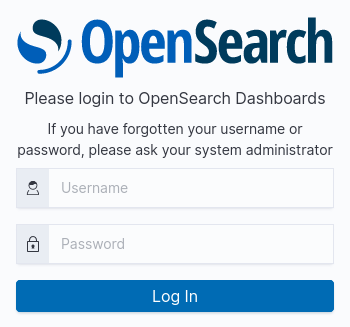
\includegraphics[width=0.4\textwidth]{Figures/opensearch-dashboards-login}
    \decoRule
    \caption[OpenSearch Dashboards (\emph{Login})]{Página de \emph{login} en OpenSearch Dashboards}
    \label{fig:opensearch-dashboards-login}
\end{figure}

\section{Ejemplo de uso}

Para ilustrar el funcionamiento de Grimoirebots, en esta sección se va a mostrar un caso de uso en el que un usuario quiere analizar una serie de repositorios git\index{Git}, y después visualizar los datos generados en este análisis.

Para ello se va a hacer uso de la herramienta \nameref{sec:postman}\index{Postman}, que permite realizar fácilmente peticiones HTTP\index{HTTP} a diferentes \emph{endpoints}.

\subsection{Creación de una petición de análisis}

El primer paso será realizar una petición POST al \emph{endpoint} \code{http://localhost:8000/\\orders/}, con la configuración del análisis en el campo \emph{body} de la solicitud (Figura~\ref{fig:example1}).

\begin{figure}[ht]
    \centering
    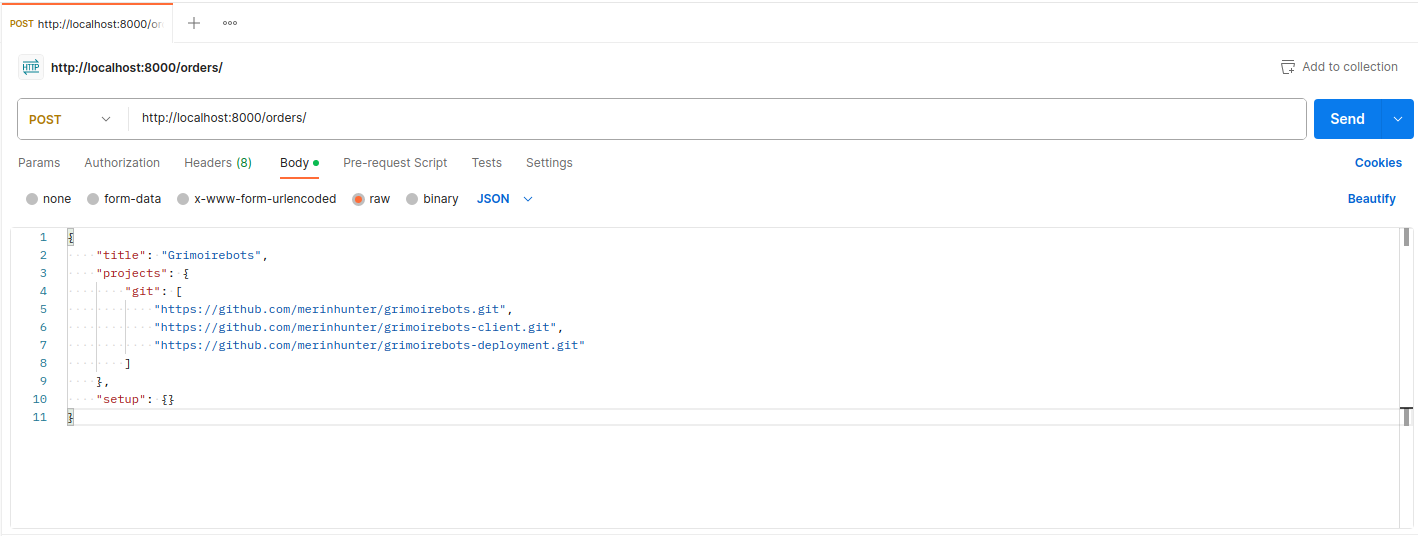
\includegraphics[width=\textwidth]{Figures/example1}
    \decoRule
    \caption[Grimoirebots (Creación de análisis)]{Creación de una solicitud de análisis en Grimoirebots}
    \label{fig:example1}
\end{figure}

La solicitud dará como respuesta un \textbf{201 Created} (Figura~\ref{fig:example2}).

\begin{figure}[ht]
    \centering
    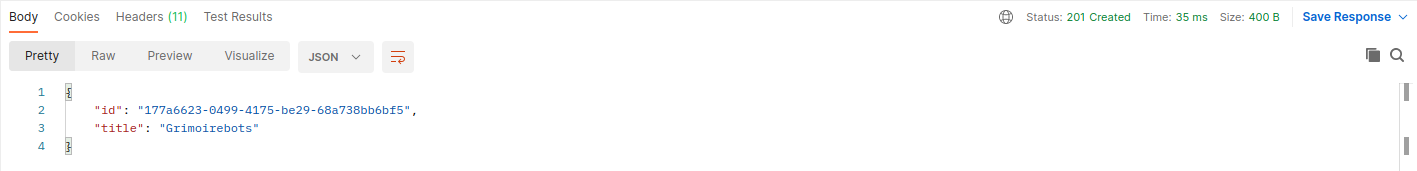
\includegraphics[width=\textwidth]{Figures/example2}
    \decoRule
    \caption[Grimoirebots (Respuesta de creación de análisis)]{Respuestas a la creación de una solicitud de análisis en Grimoirebots}
    \label{fig:example2}
\end{figure}

Si se realiza una petición GET al \emph{endpoint} \code{http://localhost:8000/orders/\\<order\_id>}, sustituyendo \code{<order\_id>} por el identificador de la solicitud de análisis enviada, se puede obtener el objeto creado (Figura~\ref{fig:example3}).

\begin{figure}[ht]
    \centering
    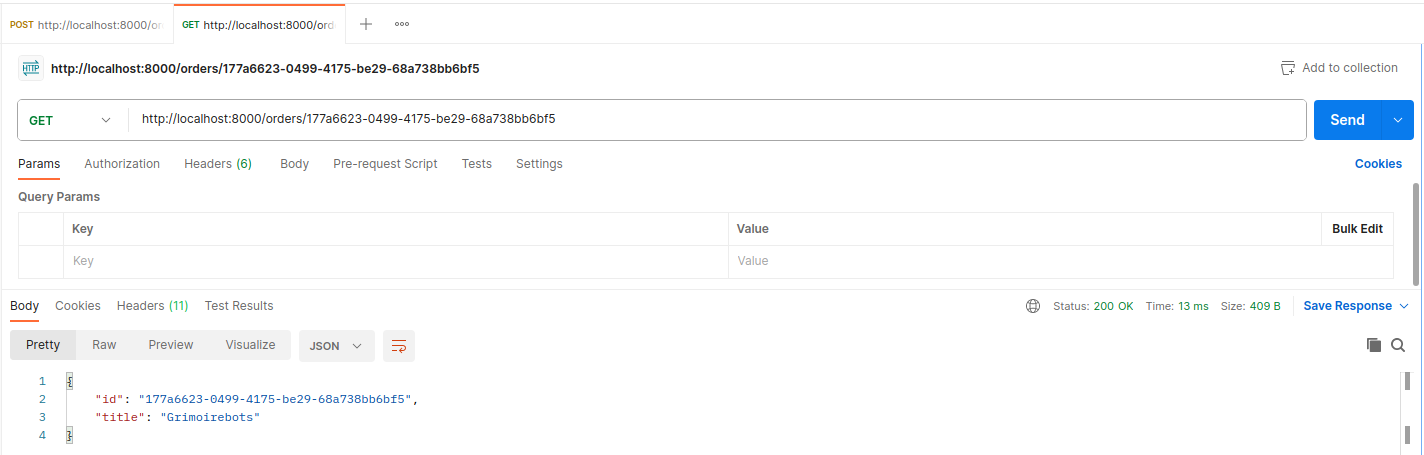
\includegraphics[width=\textwidth]{Figures/example3}
    \decoRule
    \caption[Grimoirebots (Solicitud de análisis)]{Solicitud de análisis en Grimoirebots}
    \label{fig:example3}
\end{figure}

Y realizando una petición GET a los \emph{endpoints} \code{http://localhost:8000/orders/\\<order\_id>/projects.json} y \code{http://localhost:8000/orders/<order\_id>/\\setup.cfg} se pueden obtener los ficheros de configuración de \nameref{sec:grimoirelab}\index{GrimoireLab} para el análisis (Figura~\ref{fig:example4} y Figura~\ref{fig:example5}).

\begin{figure}[ht]
    \centering
    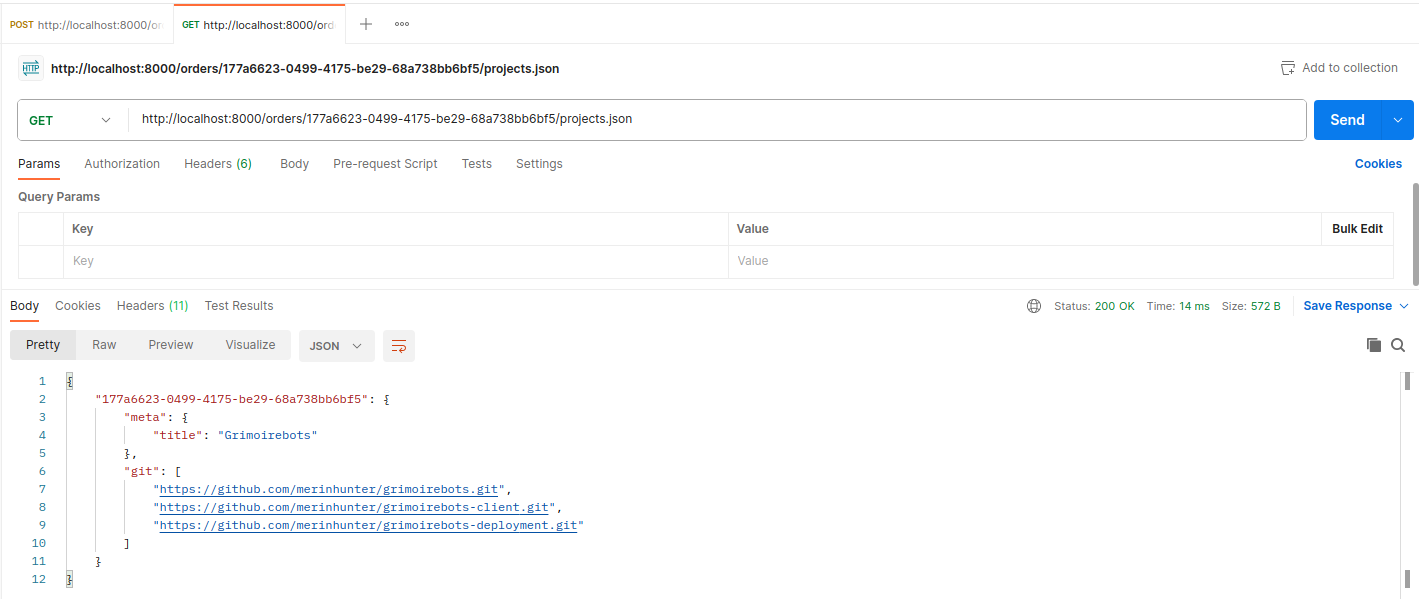
\includegraphics[width=\textwidth]{Figures/example4}
    \decoRule
    \caption[Análisis en Grimoirebots (Fichero de repositorios)]{Fichero de repositorios de un análisis en Grimoirebots}
    \label{fig:example4}
\end{figure}

\begin{figure}[ht]
    \centering
    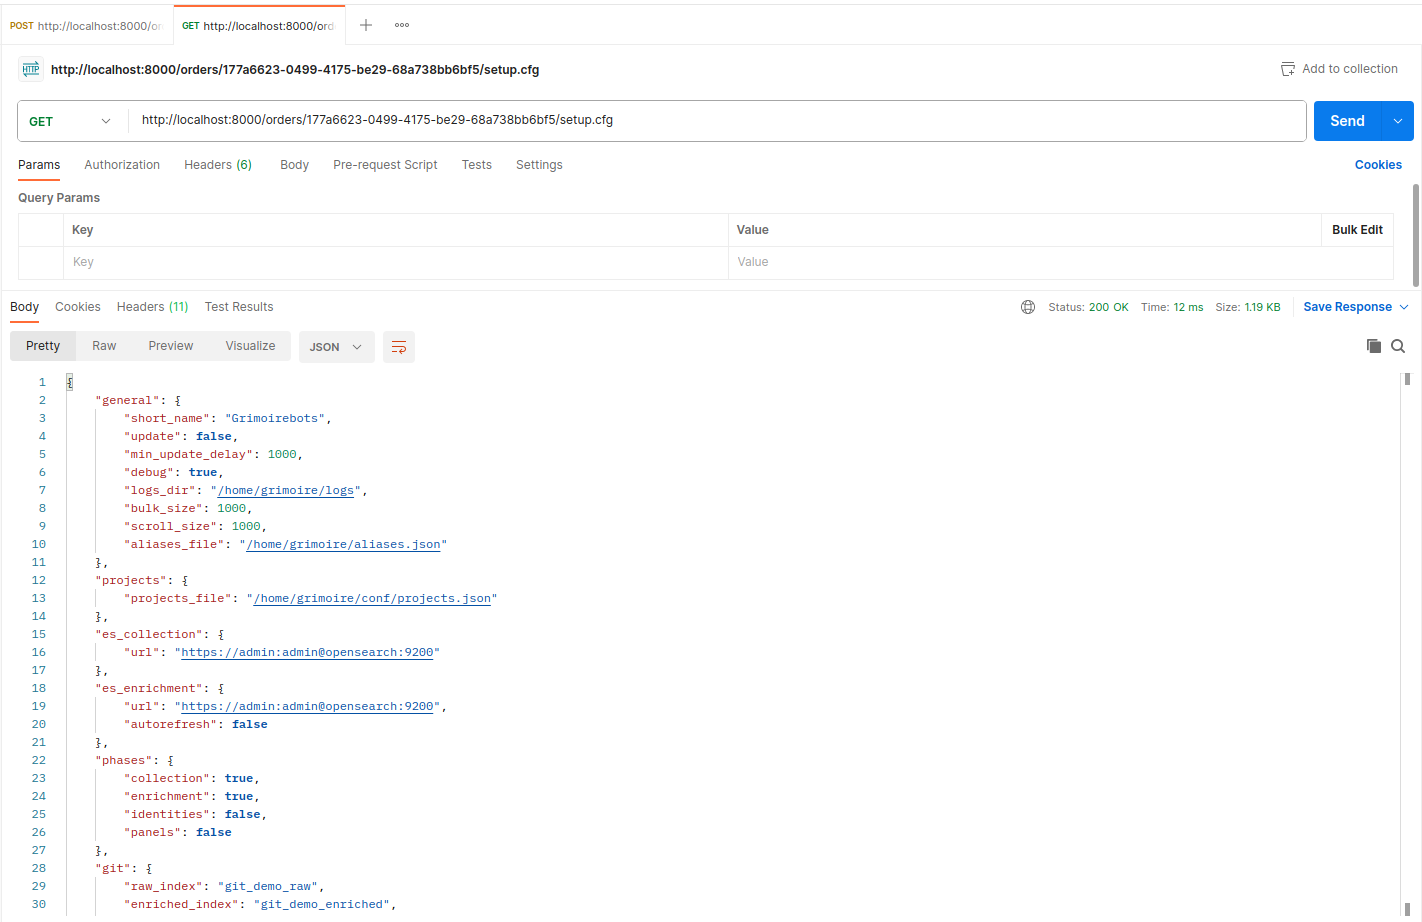
\includegraphics[width=\textwidth]{Figures/example5}
    \decoRule
    \caption[Análisis en Grimoirebots (Fichero de configuración)]{Fichero de configuración de un análisis en Grimoirebots}
    \label{fig:example5}
\end{figure}

A continuación, el cliente de Grimoirebots solicitará al servidor estos ficheros. Se pueden comprobar los logs del contenedor para asegurarnos de ello:

\begin{lstlisting}[language=bash]
$ docker logs grimoirebots-client
2023-06-18 17:00:54,511 - INFO - Retrieving pending orders from http://localhost:8000
2023-06-18 17:00:54,523 - INFO - Retrieved 1 orders
2023-06-18 17:00:54,523 - INFO - Processing order 177a6623-0499-4175-be29-68a738bb6bf5
2023-06-18 17:00:54,523 - INFO - Retrieving projects.json for order 177a6623-0499-4175-be29-68a738bb6bf5
2023-06-18 17:00:54,536 - INFO - File projects.json for order 177a6623-0499-4175-be29-68a738bb6bf5 saved at reports/177a6623-0499-4175-be29-68a738bb6bf5/projects.json
2023-06-18 17:00:54,536 - INFO - Retrieving setup.cfg for order 177a6623-0499-4175-be29-68a738bb6bf5
2023-06-18 17:00:54,550 - INFO - File setup.cfg for order 177a6623-0499-4175-be29-68a738bb6bf5 saved at reports/177a6623-0499-4175-be29-68a738bb6bf5/setup.cfg
2023-06-18 17:00:54,550 - INFO - Starting GrimoireLab container
2023-06-18 17:00:54,676 - INFO - Analysis for 177a6623-0499-4175-be29-68a738bb6bf5 has finished
2023-06-18 17:00:54,676 - INFO - Creating report for order 177a6623-0499-4175-be29-68a738bb6bf5
2023-06-18 17:00:54,690 - INFO - Report 9ddf60a6-964f-41d5-9493-f058cbdc2c41 created for order 177a6623-0499-4175-be29-68a738bb6bf5
\end{lstlisting}

Y una vez que el cliente haya comenzado el análisis, se puede realizar una petición GET al \emph{endpoint} \code{http://localhost:8000/reports/} para comprobar que existe un informe asociado a la petición inicial (Figura~\ref{fig:example6}).

\begin{figure}[ht]
    \centering
    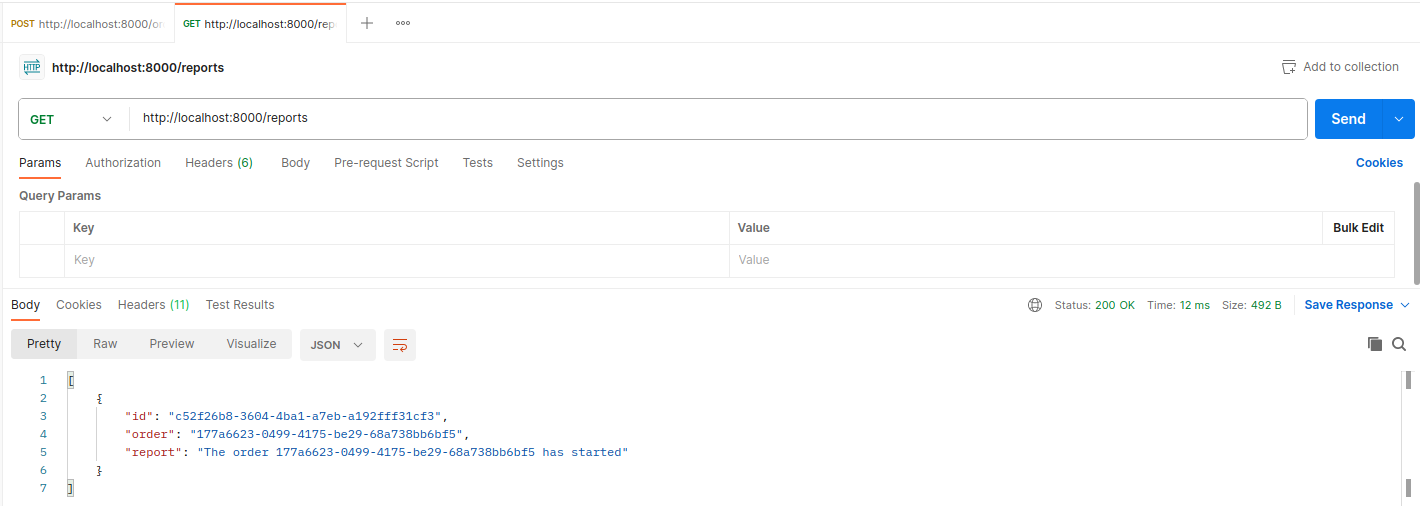
\includegraphics[width=\textwidth]{Figures/example6}
    \decoRule
    \caption[Grimoirebots (Informe)]{Informe en Grimoirebots}
    \label{fig:example6}
\end{figure}

A partir de este momento, el análisis se está llevando a cabo en un contenedor de \nameref{sec:grimoirelab}\index{GrimoireLab}. El seguimiento de este análisis se puede realizar revisando en tiempo real los logs del contenedor, necesitando localizar a este primero:

\begin{lstlisting}[language=bash]
$ docker ps
CONTAINER ID   IMAGE    ...    NAMES
b0a1f6acf822   grimoirelab/grimoirelab:0.10.0 ... grimoirelab-177a6623-0499-4175-be29-68a738bb6bf5
...

$ docker logs -f grimoirelab-177a6623-0499-4175-be29-68a738bb6bf5
2023-06-18 17:00:55,882 - sirmordred.sirmordred - INFO -
2023-06-18 17:00:55,882 - sirmordred.sirmordred - INFO - ----------------------------
2023-06-18 17:00:55,882 - sirmordred.sirmordred - INFO - Starting SirMordred engine ...
2023-06-18 17:00:55,882 - sirmordred.sirmordred - INFO - ----------------------------
2023-06-18 17:00:55,885 - urllib3.connectionpool - DEBUG - Starting new HTTPS connection (1): localhost:9200
...
\end{lstlisting}

\subsection{Visualización de datos en OpenSearch}

Una vez que el análisis con \nameref{sec:grimoirelab}\index{GrimoireLab} haya concluido, es posible visualizar los datos del análisis y construir gráficos y métricas con ellos accediendo a \nameref{sec:opensearch}\index{OpenSearch} Dashboards. Este servicio debería estar disponible navegando a la dirección \code{http://\\localhost:5601} con un navegador web.

Las credenciales por defecto son \textbf{admin} para el usuario y la contraseña. Al acceder, lo primero que se pedirá es seleccionar el \emph{tenant} de trabajo. Para el ejemplo se seleccionará el \emph{tenant} global (Figura~\ref{fig:opensearch-tenant}).

\begin{figure}[ht]
    \centering
    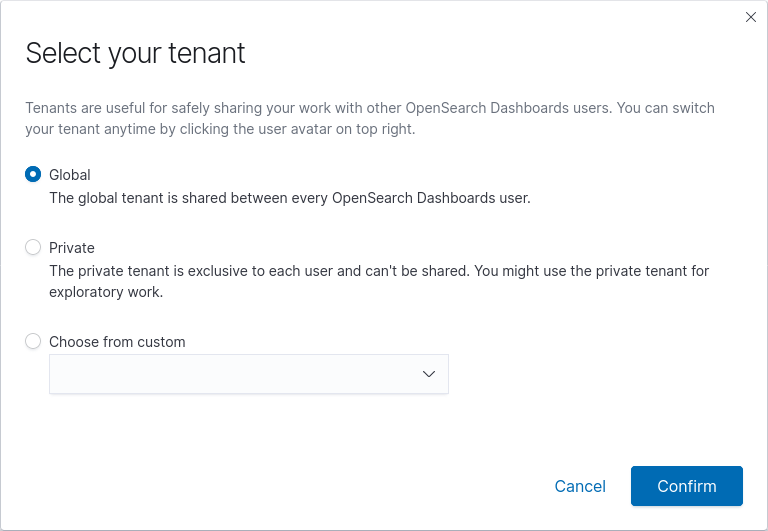
\includegraphics[width=\textwidth]{Figures/opensearch-tenant.png}
    \decoRule
    \caption[OpenSearch (Selección de \emph{tenant})]{Selección de \emph{tenant} en OpenSearch}
    \label{fig:opensearch-tenant}
\end{figure}

Si se accede a la sección \code{Index Management / Indices} es posible comprobar que existen algunos índices originados por \nameref{sec:grimoirelab}\index{GrimoireLab}, como \code{git\_demo\_raw} o \code{git\_demo\_\\enriched} (Figura~\ref{fig:opensearch-indices}).

\begin{figure}[ht]
    \centering
    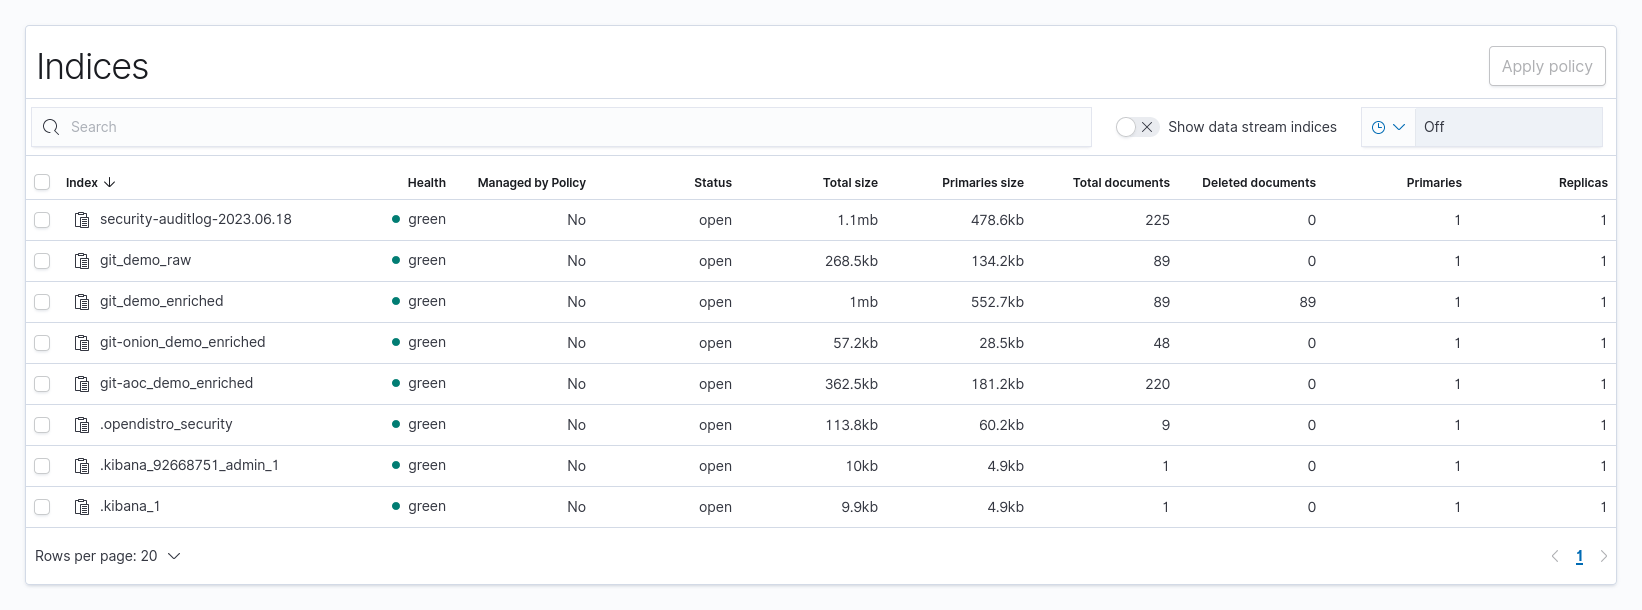
\includegraphics[width=\textwidth]{Figures/opensearch-indices.png}
    \decoRule
    \caption[OpenSearch (Índices)]{Índices en OpenSearch}
    \label{fig:opensearch-indices}
\end{figure}

Para visualizar los datos, es necesario primero crear un \emph{index pattern}. Esto sirve para que \nameref{sec:opensearch}\index{OpenSearch} sepa qué campos de los documentos debe utilizar en la indexación de la información. Para ello, se debe hacer clic en la pestaña \emph{Discover}, en la barra lateral, desde donde se solicitará la creación de un \emph{index pattern}. Para este ejemplo se utilizará como \emph{index pattern} el valor \code{git}, que concuerda con uno de los índices existentes (Figura~\ref{fig:opensearch-index-pattern-creation}).

\begin{figure}[ht]
    \centering
    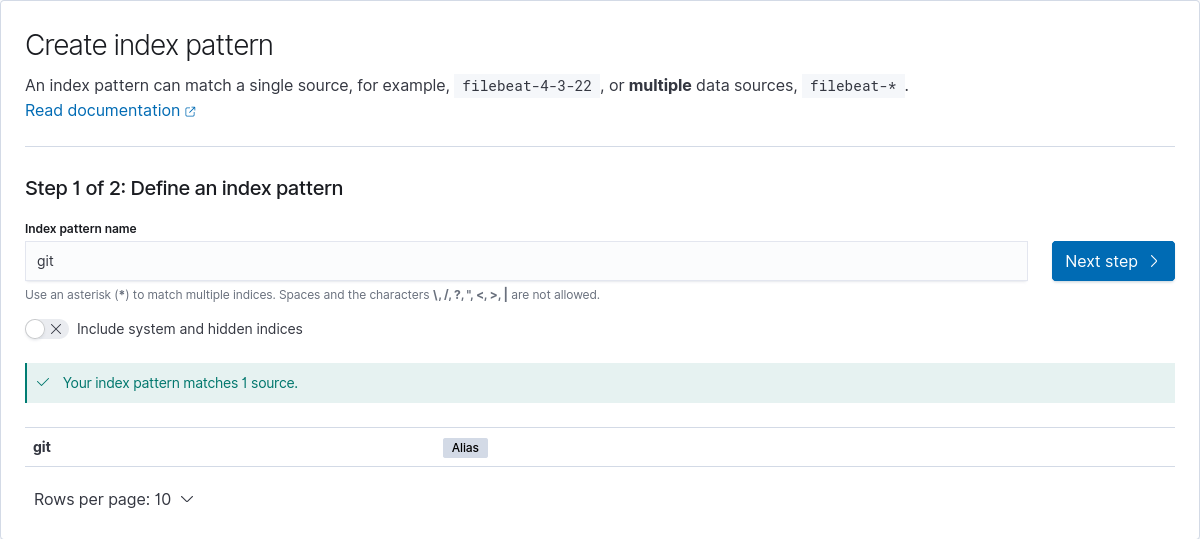
\includegraphics[width=\textwidth]{Figures/opensearch-index-pattern-creation.png}
    \decoRule
    \caption[OpenSearch (Creación de \emph{Index Pattern})]{Creación de \emph{Index Pattern} en OpenSearch}
    \label{fig:opensearch-index-pattern-creation}
\end{figure}

Como campo temporal se utilizará el campo \code{utc\_commit}, que corresponde con la hora UTC en la que cada \emph{commit} se realizó (Figura~\ref{fig:opensearch-index-pattern-timestamp}).

\begin{figure}[ht]
    \centering
    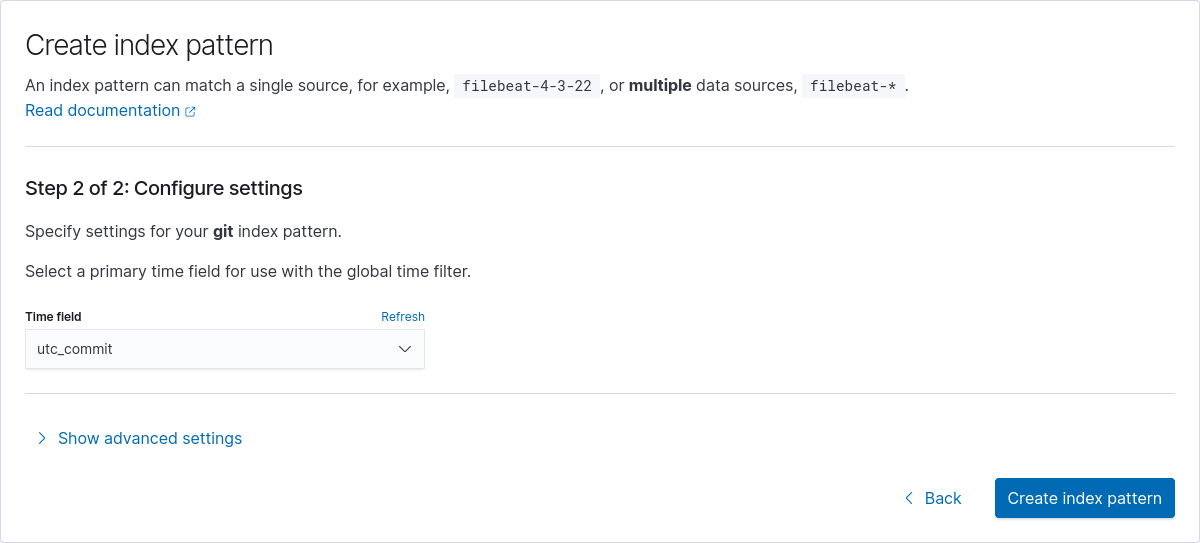
\includegraphics[width=\textwidth]{Figures/opensearch-index-pattern-timestamp.png}
    \decoRule
    \caption[OpenSearch (Creación de \emph{Index Pattern}) Cont.]{Creación de \emph{Index Pattern} en OpenSearch (Cont.)}
    \label{fig:opensearch-index-pattern-timestamp}
\end{figure}

Una vez creado el \emph{index pattern}, es posible hacer clic en \emph{Discover} y visualizar algunos de los datos generados por el análisis. Si se ajusta la fecha al último año, se obtiene una serie temporal con los \emph{commits} realizados en los diferentes repositorios analizados a lo largo del último año (Figura~\ref{fig:opensearch-discover}).

\begin{figure}[ht]
    \centering
    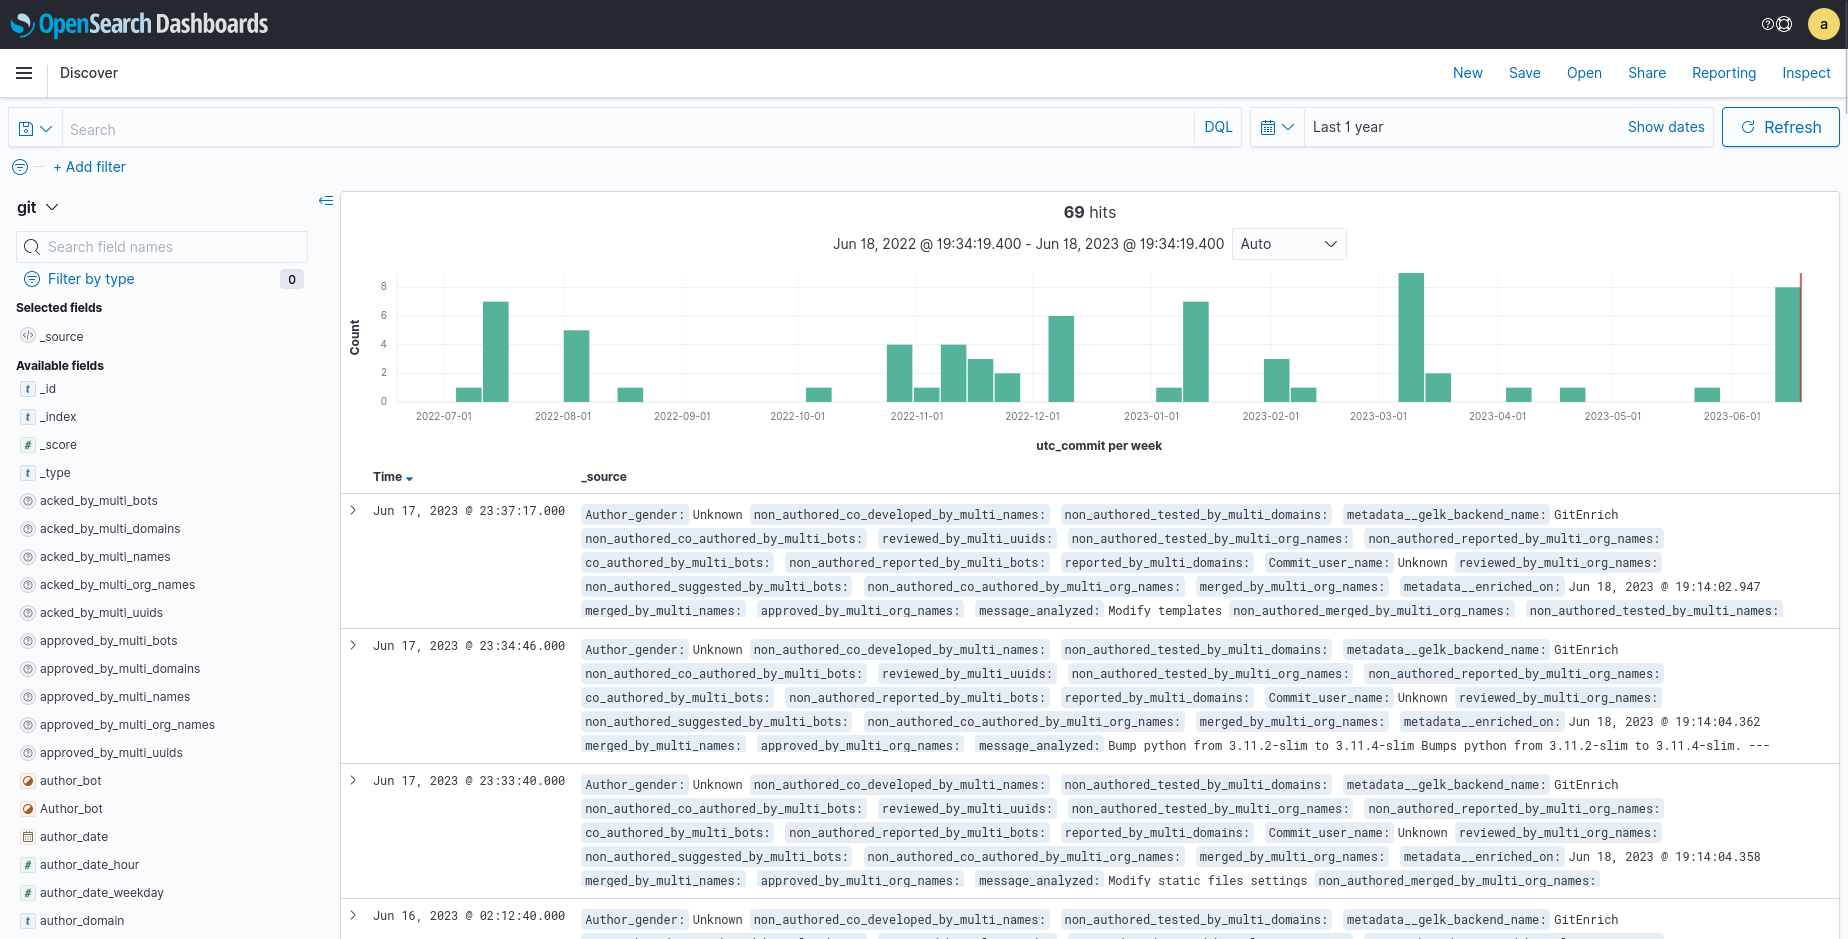
\includegraphics[width=\textwidth]{Figures/opensearch-discover.png}
    \decoRule
    \caption[OpenSearch (Sección \emph{Discover})]{Sección \emph{Discover} en OpenSearch}
    \label{fig:opensearch-discover}
\end{figure}
